\subsection{RSS3 \glsfmtfull{GI}}
\label{subsec:GI}

{
    \begin{figure}[tb!]
        \centering
        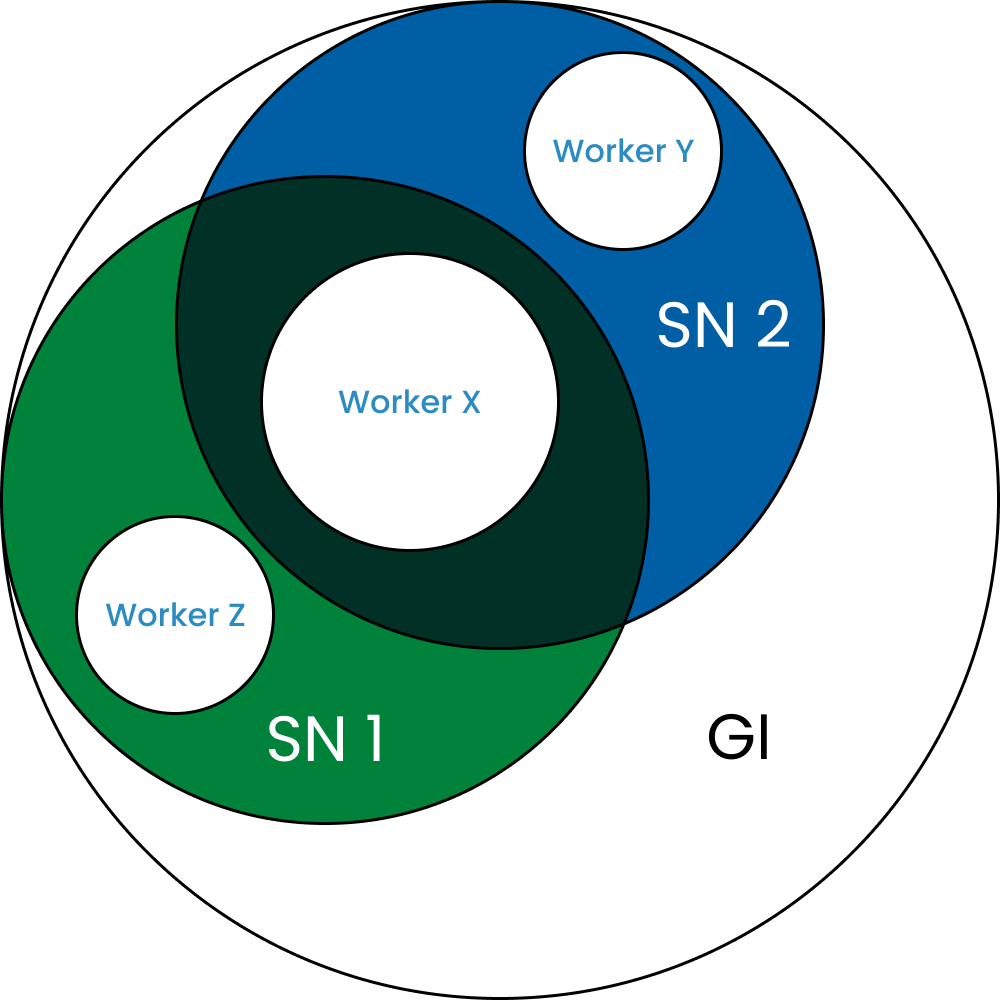
\includegraphics[width=0.7\columnwidth]{figures/GI.png}
        \caption{A Venn diagram illustrating the relationship between the worker, the \glsfmtlong{Node}, and the \glsfmtlong{GI}.}
        \label{fig:GI}
    \end{figure}
}

A \gls{GI} is responsible for facilitating coordination among \glspl{Node} and engaging with the \gls{VSL} and performs critical functions to ensure the \gls{DSL} is robust and reliable.

Given the importance of the \gls{GI} to the Network, its operation is subject to a set of stringent requirements imposed by the Network.

\subsubsection{Performance Assurance} A GI acts as a load balancer and query router for end users to retrieve information from \glspl{Node}.
The unique architecture of the \gls{DSL} demands \glspl{GI} to be equipped with more computational capabilities to work out the optimal route for end users to retrieve specific information from \gls{Node} and frequently from a group of \glspl{Node} simultaneously.

\subsubsection{Quality Assurance} A GI acts as a supervisor for \glspl{Node} to ensure the quality of service.
With the \gls{DSL} being a permissionless Sublayer, the quality needs to be maintained strictly to ensure \glsfmtlong{R3N}'s robustness and reliability.
A \gls{GI} monitors the quality of \glspl{Node} and slashes the \gls{Node} if it fails to meet the requirements.

\subsubsection{Proof Onchain} A GI keeps track of the work and slash records of \glspl{Node} and submits them to the \gls{VSL} for settlement and reward allocation.

\subsection{Reliability Score}

A \gls{GI} routes requests to \glspl{Node} based on their information coverage and a \gls{RS}.
The calculation of \reliabilityScore\ is based on a range of factors, including but not limited to the \gls{Node}'s uptime, work, slash records, operation deposit, and staking/trust pool size.
\glspl{Node} with a higher \reliabilityScore\ have an increased likelihood of receiving requests.
